\documentclass[bibliography=totocnumbered]{scrartcl}
\usepackage{imakeidx}
\usepackage{ragged2e}
\usepackage{setspace} % Um den Zeilenabstand zu ändern.
\usepackage{gensymb}
%\usepackage{authblk}
% \usepackage{minitoc} % for the chpaters
\usepackage{wasysym}
%\usepackage{SI}
\usepackage{array} % Verwendung von Matrizen
\usepackage{booktabs} % Schöne Tabellen beziehungsweise sie sehen damit professioneller aus.
\usepackage{tabulary} % Ähnlich wie tabularx, ermöglicht aber das ändern der Ausrichtung der Spalten.
\usepackage{tabularx} % Tabellen mit automatischen Zeilenumbruch.
\usepackage{enumitem}
\usepackage{physics}
\usepackage[T1]{fontenc}% fontec und inputenc ermöglichen
\usepackage{graphicx}%Für Grafiken
\usepackage{rotating} % lässt Grafiken rotieren
\usepackage{mathtools}% mathematische Werkzeuge
\usepackage{amsmath}% Mathetools
\usepackage{amsfonts}% Mathetools
\usepackage{amssymb}% Symbole wie Natürliche Zahlen
\usepackage{geometry}
%\usepackage{bibtex} 
\usepackage{tablefootnote}% Fußnoten in Tabellen
\usepackage{float}% für eingebundene Bilder
\usepackage{fancyhdr} % Seiten schöner gestalten, insbesondere Kopf- und Fußzeile
\usepackage{ulem} 
\usepackage{dcolumn}% Align table columns on decimal point
\usepackage{bm}% bold math
\usepackage[ngerman]{babel} % Worttrennung nach der neuen Rechtschreibung und deutsche Bezeichnungen. babelfunktion wird wegen Literatur gebraucht.
\usepackage{subfloat} % Was macht diese Packet?
\usepackage{caption} % Unter-/Überschriften für Bilder, Grafiken und Tabellen
\usepackage{subcaption}
\usepackage{txfonts}
\usepackage{titling}% Titel
\usepackage[style=alphabetic]{biblatex} %biblatex mit alphabetic laden. alphbetic=Zitationsstil
\usepackage{bookmark}
\usepackage[printonlyused]{acronym}
\usepackage{amsthm}
\usepackage{pdfpages}
\usepackage{tikz}
\usepackage[siunitx,americanvoltages, europeanresistors,americancurrents]{circuitikz}
\usepackage{listings}
\usepackage{abstract}
\usepackage[per-mode = fraction]{siunitx}
\usepackage{hyperref}
\newcommand{\R}{\mathbb{R}} % reelle Zahlen
\newcommand{\N}{\mathbb{N}} % natürliche Zahlen
\newcommand{\C}{\mathbb{C}} % komplexe Zahlen
\newcommand{\Q}{\mathbb{Q}} % rationale Zahlen
\newcommand{\Z}{\mathbb{Z}} % ganze Zahlen
\newcommand{\F}{\mathbf{F}} % Kraft
\newcommand{\E}{\mathbf{E}} % Energie
\newcommand{\V}{\mathbf{v}} % Geschwindigkeit
\newcommand{\B}{\mathbf{B}} % magnetischer Fluss
\newcommand{\J}{\mathbf{j}} % Stromdichte ?
\newcommand{\D}{\mathbf{D}} % elektrische Induktion
\newcommand{\HH}{\mathbf{H}} % magnetische Feldstärke
\newcommand{\M}{\mathbf{M}} % Magnetisierung
\newcommand{\p}{\mathbf{P}}
\newcommand{\rr}{\mathbf{r}}
\newcommand{\vp}{\varphi}
\newcommand{\ve}{\varepsilon}
\newcommand{\vcc}[1]{\left(\begin{matrix}#1\end{matrix}  \right)}
\newcommand{\m}[1]{\left\lbrace #1\right\rbrace}
\newcommand{\los}{\noindent\textbf{Lösung}:}
\newcommand{\rang}[2]{\text{Rang}(#1)=#2}
\newcommand{\vpe}{\frac{1}{4\pi\ve_0}}
\newcommand{\qvpe}{\frac{q}{4\pi\ve_0}}
\newcommand{\geg}{\ac{geg.}}
\newcommand{\ges}{\ac{ges.}}

\newcommand{\kommando}[1]{$\backslash$\textit{#1}}
\newcommand{\com}[1]{$\backslash$\textit{#1}$\left\lbrace\ldots\right\rbrace$}
\newcommand{\Com}[2]{$\backslash$\textit{#1}$\left\lbrace #2\right\rbrace$}
\newcommand{\NeuKommando}[2]{$\backslash \textit{#1} \left\lbrace \backslash \textit{#2}\right\rbrace$}
\newcommand{\latex}{\LaTeX $\;$}


% si unitx
\DeclareSIUnit\litre{l}

\hypersetup{
	colorlinks=true,
	linkcolor=blue,
	filecolor=magenta,      
	urlcolor=cyan,
	citecolor=lime!50!black,
	filecolor=red
}
%\addbibresource{} %Bibliographiedateien laden
\addbibresource{bib.bib}

\geometry{a4paper, left=25mm, right=25mm, top=30mm, bottom=30mm}
\lhead{\thedate}
\rhead{GPR}
\lhead{\thetitle}
\pagestyle{fancy}

\usetikzlibrary{patterns}
\usetikzlibrary{3d}
\makeindex[title=Stichwortverzeichnis,intoc
,options= -s Index-Formatierung.ist
]
\author{Ben J. F.}
\allowdisplaybreaks

\lstset
{ %Formatting for code in appendix
    basicstyle=\footnotesize,
    numbers=left,
    stepnumber=1,
    showstringspaces=false,
    tabsize=2,
    breaklines=true,
    breakatwhitespace=false,
}

\date{03.08.2021}

\title{M10 - Gyroskop}

\rfoot{M10}

\begin{document}
	\newgeometry{left=14mm, right=13.5mm, top=60mm, bottom=30mm}
	\begin{titlepage}
		\begin{center}
			{\huge{Grundpraktikum}}\\\vspace*{15mm}
			{\huge{\textbf{\thetitle}}}\\\vspace*{20mm}
			{\theauthor}\\\vspace*{10mm}
			{\thedate}\\\vspace*{20mm}
			\vspace{1.5cm}
			\begin{abstract}
				In der Natur und in der Technik kommen starre rotierende Körper vor, welche man allgmein als Kreisel bezeichnet. Für den Versuch führen wir den Trägheitstensor ein, der mit den Elementen der Hauptdiagonalen, auch Haupträgheitsmomente genannt, die Bewegung eines symmetrischen Kreisels beschreibt. Um die Hauptträgheitsmomente experimentel zu bestimmen, wurden drei verschiedene Methoden verwendet:
				
				\begin{table}[ht!]
					\centering
					\begin{tabular}{|c|c|c|}
					\hline
					Methode & Experimentatorin & Experimentator \\
					\hline
					Präzesion (gewichtet gemittelt) $ J_{x}$ [kg m$ ^{2} $] & $(2.477 \pm0.029)\cdot 10^{-3} $ & $ (2.37\pm0.11)\cdot 10^{-3} $ \\
					\hline
					Nutation $ J_{s} $ [kg m$ ^{2} $]& $(8.7 \pm0.3 )\cdot 10^{-3}$ & $(10.3 \pm1.2)\cdot 10^{-3} $ \\
					\hline
					Berechnung $ J_{x} $ [kg m$ ^{2} $]& $(3.097 \pm 0.009)\cdot 10^{-3}$ & $ (2.671\pm 0.009)\cdot 10^{-3}$ \\
					\hline
				\end{tabular}
				\end{table}
			
			\end{abstract}
			
			
		\end{center}
	\end{titlepage}
	\makeatother
	\restoregeometry
	\newpage
	
	\tableofcontents
	\newpage
	\listoffigures 
	\listoftables
	\newpage
	
	
	
	\section{Motivation und theoretische Vorbetrachtungen}
Ziel des Experimentes war es die Bestimmung der Hauptträgheitsmomente.
Dafür wird am Ende eines Wagenbalken ein Kreisel angebracht, so dass deren Achsen zusammen fällt, somit waagerecht bleibt durch Gleichgewicht. Der Kreisel wird mittels eines Motors zum Drehen gebracht mit einer Kreiseldrehzahl n.
Für den Versuch wird nun auf der anderem Ende zum Kreisel ein Gewicht, wodurch ein zusätzliches ein Drehmoment erzeugt wird.
Diese Konstruktion entspricht dem Aufbau eines Gyroskops.
Allgemein gilt für das Hauptträgheitsmoment entlang der Achse die von dem Kreis zu der Masse zeigt (hier Jx benannt) mit der Präzisionperiodendauer (der Zeit die der Kreisel für eine Drehung der $ x $-Achse um 90° braucht.) und dem Drehmoment M.
\begin{align}\label{eq: Tp}
	T_{p}=\dfrac{4\pi^{2}J_{x}n}{M}
\end{align}
	Da$  M=r m g \cos(\varphi) $ gilt, mit r dem Radius des Schwepunktes zu dem Aufhängepunkt und phi den Winkel zwischen der x Achse vor und nach dem Anbringen der Masse. Durch Kleinwinkelnährung kann man $ M=rmg $ annehmen.\\\\
	Zum Messen der Trägheitsmomente gibt es mehrere Möglichkeiten.
	\subsection{In Abhängigkeit zur Masse}
	In diesem Aufbau nutzt man beim konstanten Kreiseldrehzahl mehrere Massen die man anbringt und misst die Periodendauer der Präzisionsdrehung, also der die durch das zusätzlichen Drehmoment entsteht.\\
	Hier misst man $ T_{p}/n $, da eine konstante Drehzahl schwierig zu erhalten ist.\\
	Dann bringt man verschiedene Massen in 50g Schritten von 50g bis hin zu 500g.
	
	\subsection{In Abhängigkeit zu Kreisdrehzahl}
	Für die Masse 200g wird der Kreisel mit verschiedenen Kreisdrehzahlen von 7Hz bis 16Hz.
	Dann wird die Periodendauer der Präzisiondrehung gemessen.
	
	\subsection{Nutationsbewegung}
	Bei der dritten Messung misst man die Periodendauer der Nutationsbewegung für verschiedene Kreisdrehzahlen im Bereich von 4Hz bis 12 Hz.
	Für die Nutationsperiodendauer gilt mit den beiden Hauptträgheitsmomenten zur x Achse und das Hauptträgheitsmoment senkrecht dazu:
	\begin{equation}\label{eq: Nutation}
		T_{n}=\dfrac{J_{s}}{J_{x}}\dfrac{1}{n}
	\end{equation}
	
	Daraus lässt sich dann das zweite Hauptträgheitsmoment errechnen.
	Herleitungen und der weitere Aufbau ist im Versuchsskript\smartcite{Muller.d} zu lesen.
	\newpage
	
	
	\section{Präzesion in Abhängigkeit zur Masse}
	
	\subsection{Datenauswertung}\label{sect: Datenauswertung A1}
	Die Datensätze werden mittels lineare Regression gemäß allgemeinem Praktikumsskript\smartcite{MullerPG.2007b} der Form $ y=mx+b $ graphisch ausgewertet.\\
	Daraus ergibt sich:
	\begin{equation}\label{eq: Prezäsion Drehmoment}
		y=\dfrac{T_{m}}{n}=\dfrac{T_{M}}{n}=\dfrac{a}{rg m}+b=\dfrac{a}{M}+b
	\end{equation}
Mit $ a $ der Anstieg des Graphen und b die Periodendauer bei einer unendlichen Masse.\\
	Die $ r $-Werte bezeichnen den Radius zwischen Drehachse und Massenschwerpunkt. Sie werden folgendermaßen berechnet:
	\begin{equation}\label{eq: Hebelarm radius}
		r= l-\dfrac{h}{2}
	\end{equation}  
	Wobei $ l $ die Länge des Hebelarms ist und $ h=2.5 $cm die Höhe der Massestücke ist. Die Werte für $ l $ können im Kapitel \ref{sect: Zusätliche Skizzen} nachgelesen werden.
	
		\begin{figure}[!ht]
		\centering								 
		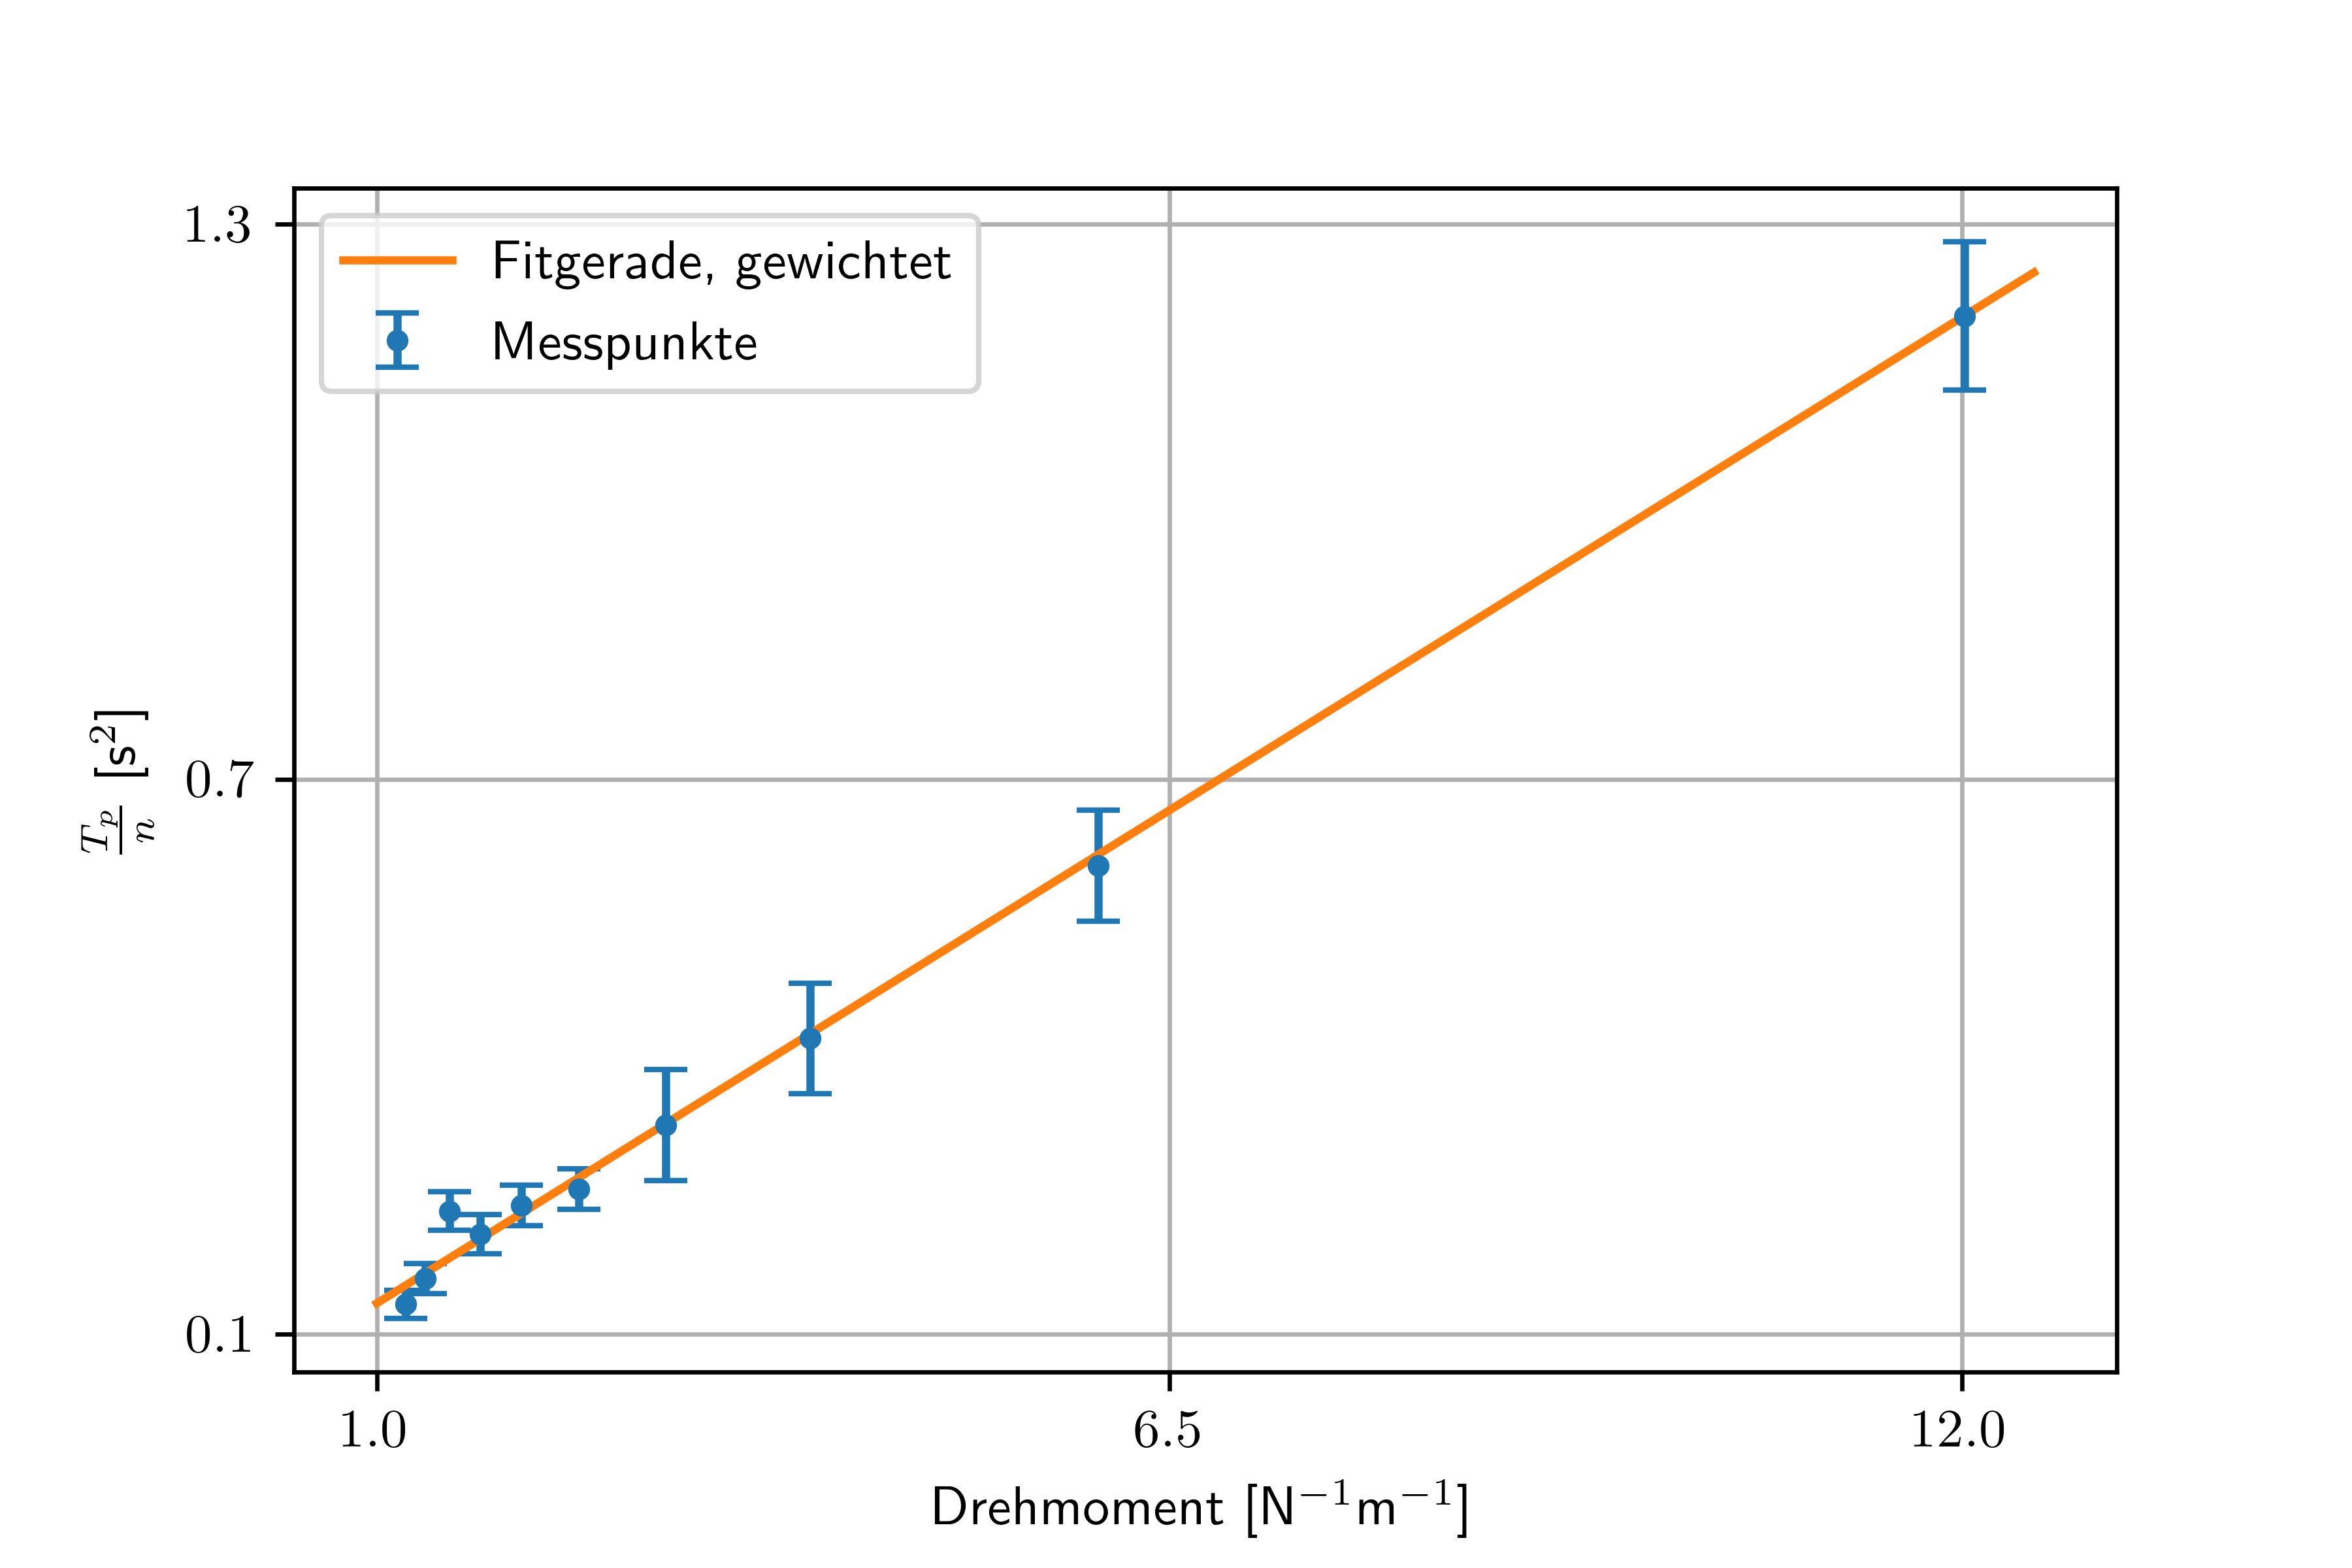
\includegraphics[width=300pt]{fotos/gpr1/A1.png}
		\caption[Präzesion in Abhängigkeit vom Drehmoment]{Präzesion in Abhängigkeit vom Drehmoment, Ben F.; $ a=0.101\pm 0.007 $ sei die Steigung, $ b=0.036\pm 0.014 $ der Achsenabschnitt, $ \chi^{2}/dof=0.39 $ Qualtität des Fits}							 
		\label{Abb: A1 Ben}							 
	\end{figure}

\newpage
\begin{figure}[!ht]
	\centering								 
	\includegraphics[width=300pt]{fotos/gpr1/M10_A1_S.png}
	\caption[Präzesion in Abhängigkeit vom Drehmoment]{Präzesion in Abhängigkeit vom Drehmoment; $ a=(52.5\pm0.7)\cdot10^{-3} $ sei die Steigung, $ b=0.52\pm0.11 $ der Achsenabschnitt, \\$ \chi^{2}/dof=0.46 $ Qualtität des Fits}							 
	\label{Abb: A1 Sara}							 
\end{figure}


	
	Der lineare Zusammenhang scheint so mit bestätigt.
	
	\subsection{Berechnung von $ J_{x} $}
	Der $ J_{x} $-Wert ergibt sich aus folgender Gleichung:
	\begin{equation}\label{eq: Jx aus Drehmoment}
		J_{x}=\dfrac{arg}{4\pi ^{2}}=\dfrac{a}{4\pi ^{2}}
	\end{equation}
Der Zähler $ arg $ gilt für die Experimentatorin und der Zähler $ a $ gilt für den Experimentator.\\
	Somit haben wir folgende Ergebnisse:
	\begin{table}[ht!]
		\centering
		\caption{Trägheitsmoment aus Drehmoment}
		\begin{tabular}{|c|c|c|}
			\hline
			& Experimentatorin & Experimentator \\
			\hline
			$ J_{x} $ [kg m$ ^{2} $]& $ ( 2.21\pm0.03  ) $ & $ (2.56\pm 0.17) $ \\
			\hline
		\end{tabular}
	\label{tab: Jx aus Kreisdrehzahl}
	\end{table}
	
	\newpage
	\section{Präzesion (Kreisdrehzahl)}
	
	\subsection{Datenauswertung}
	Bezüglich des Radius $ r $ siehe im Kapitel \ref{sect: Datenauswertung A1} nach.\\
	Damit wird die lineare Regression gemäß Material 2 der Form $ y=mx+b $.
	Daraus ergibt sich:
	\begin{equation}\label{eq: Präzesion Kreisdrehzahl}
		T_{p}=\dfrac{4\pi ^{2}J_{x}n}{M}+b=a\cdot n+b
	\end{equation}
	Mit a der Anstieg des Graphen und b die Periodendauer die ohne Kreiseldrehzahl durch die Nutationsbewegung entsteht.
	\begin{figure}[!ht]
		\centering								 
		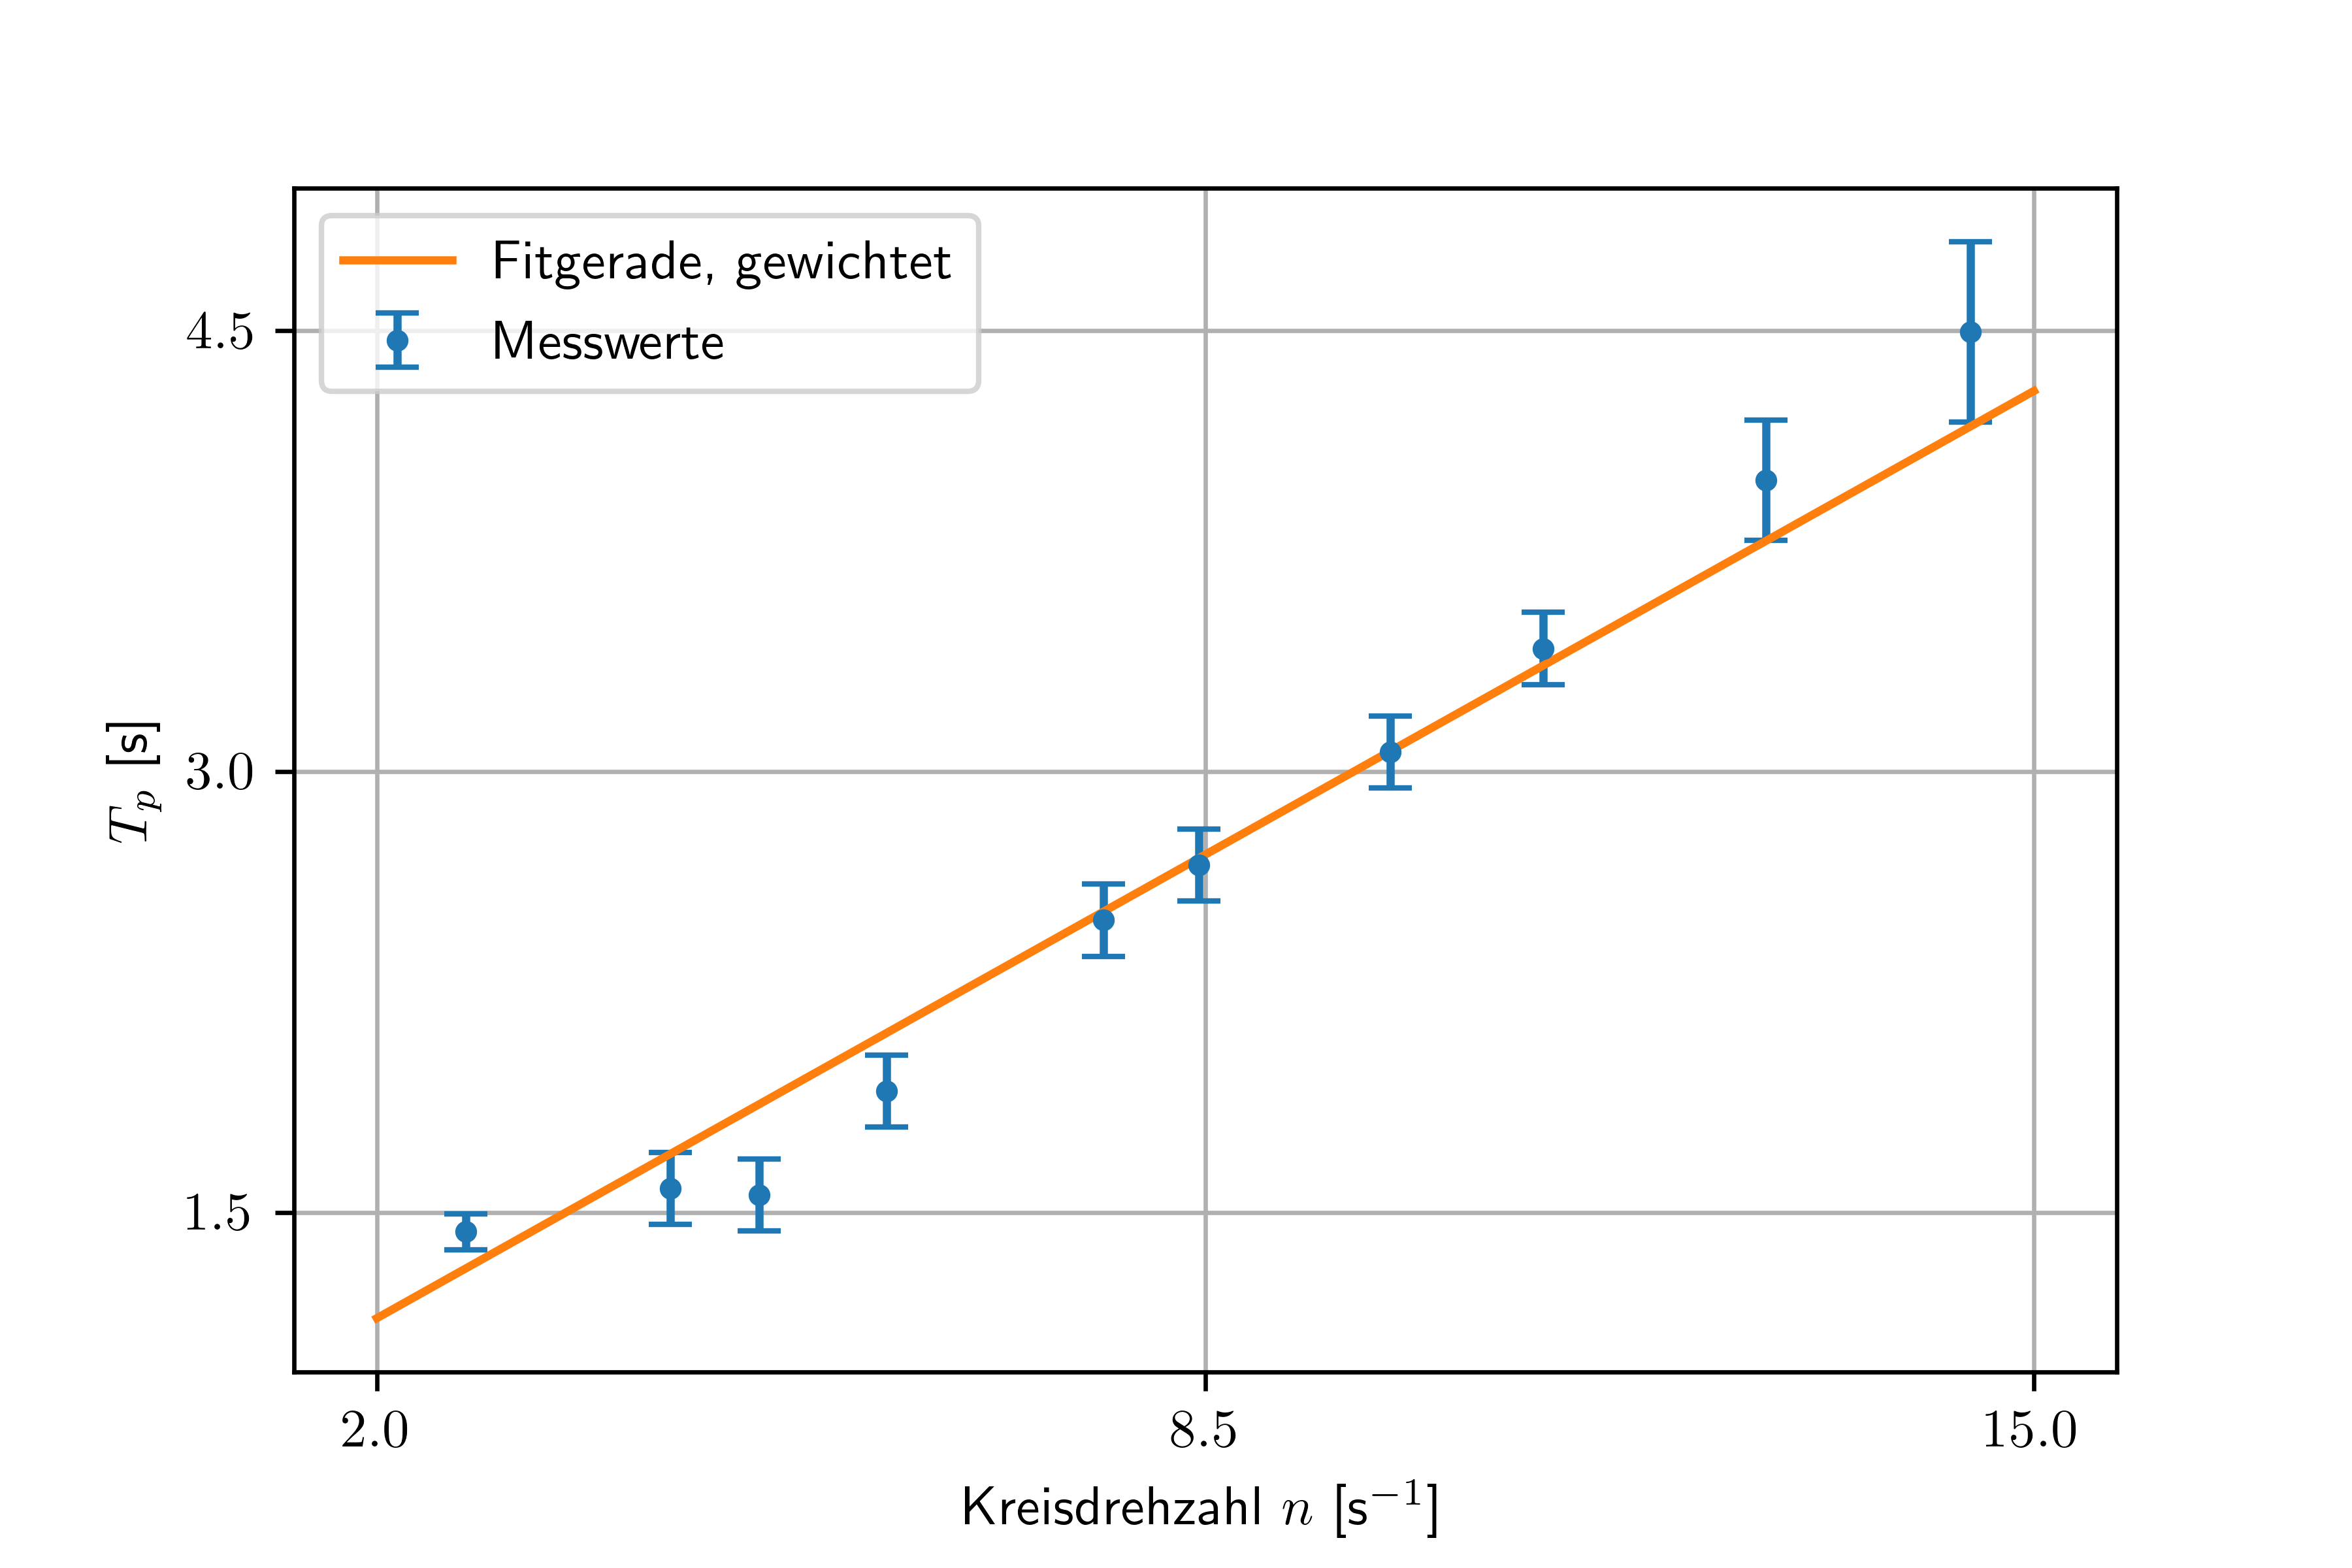
\includegraphics[width=300pt]{fotos/gpr1/A2.png}
		\caption[Präzesion in Abhängigkeit der Kreisdrehzahl]{Präzesion in Abhängigkeit vom Drehmoment, Ben F.; $ a=0.243\pm0.016 $ sei die Steigung, $ b=0.65\pm 0.11 $ der Achsenabschnitt, $ \chi^{2}/dof=0.49 $ Qualtität des Fits}							 
		\label{Abb: A2 Ben}							 
	\end{figure}


	\begin{figure}[!ht]
	\centering								 
	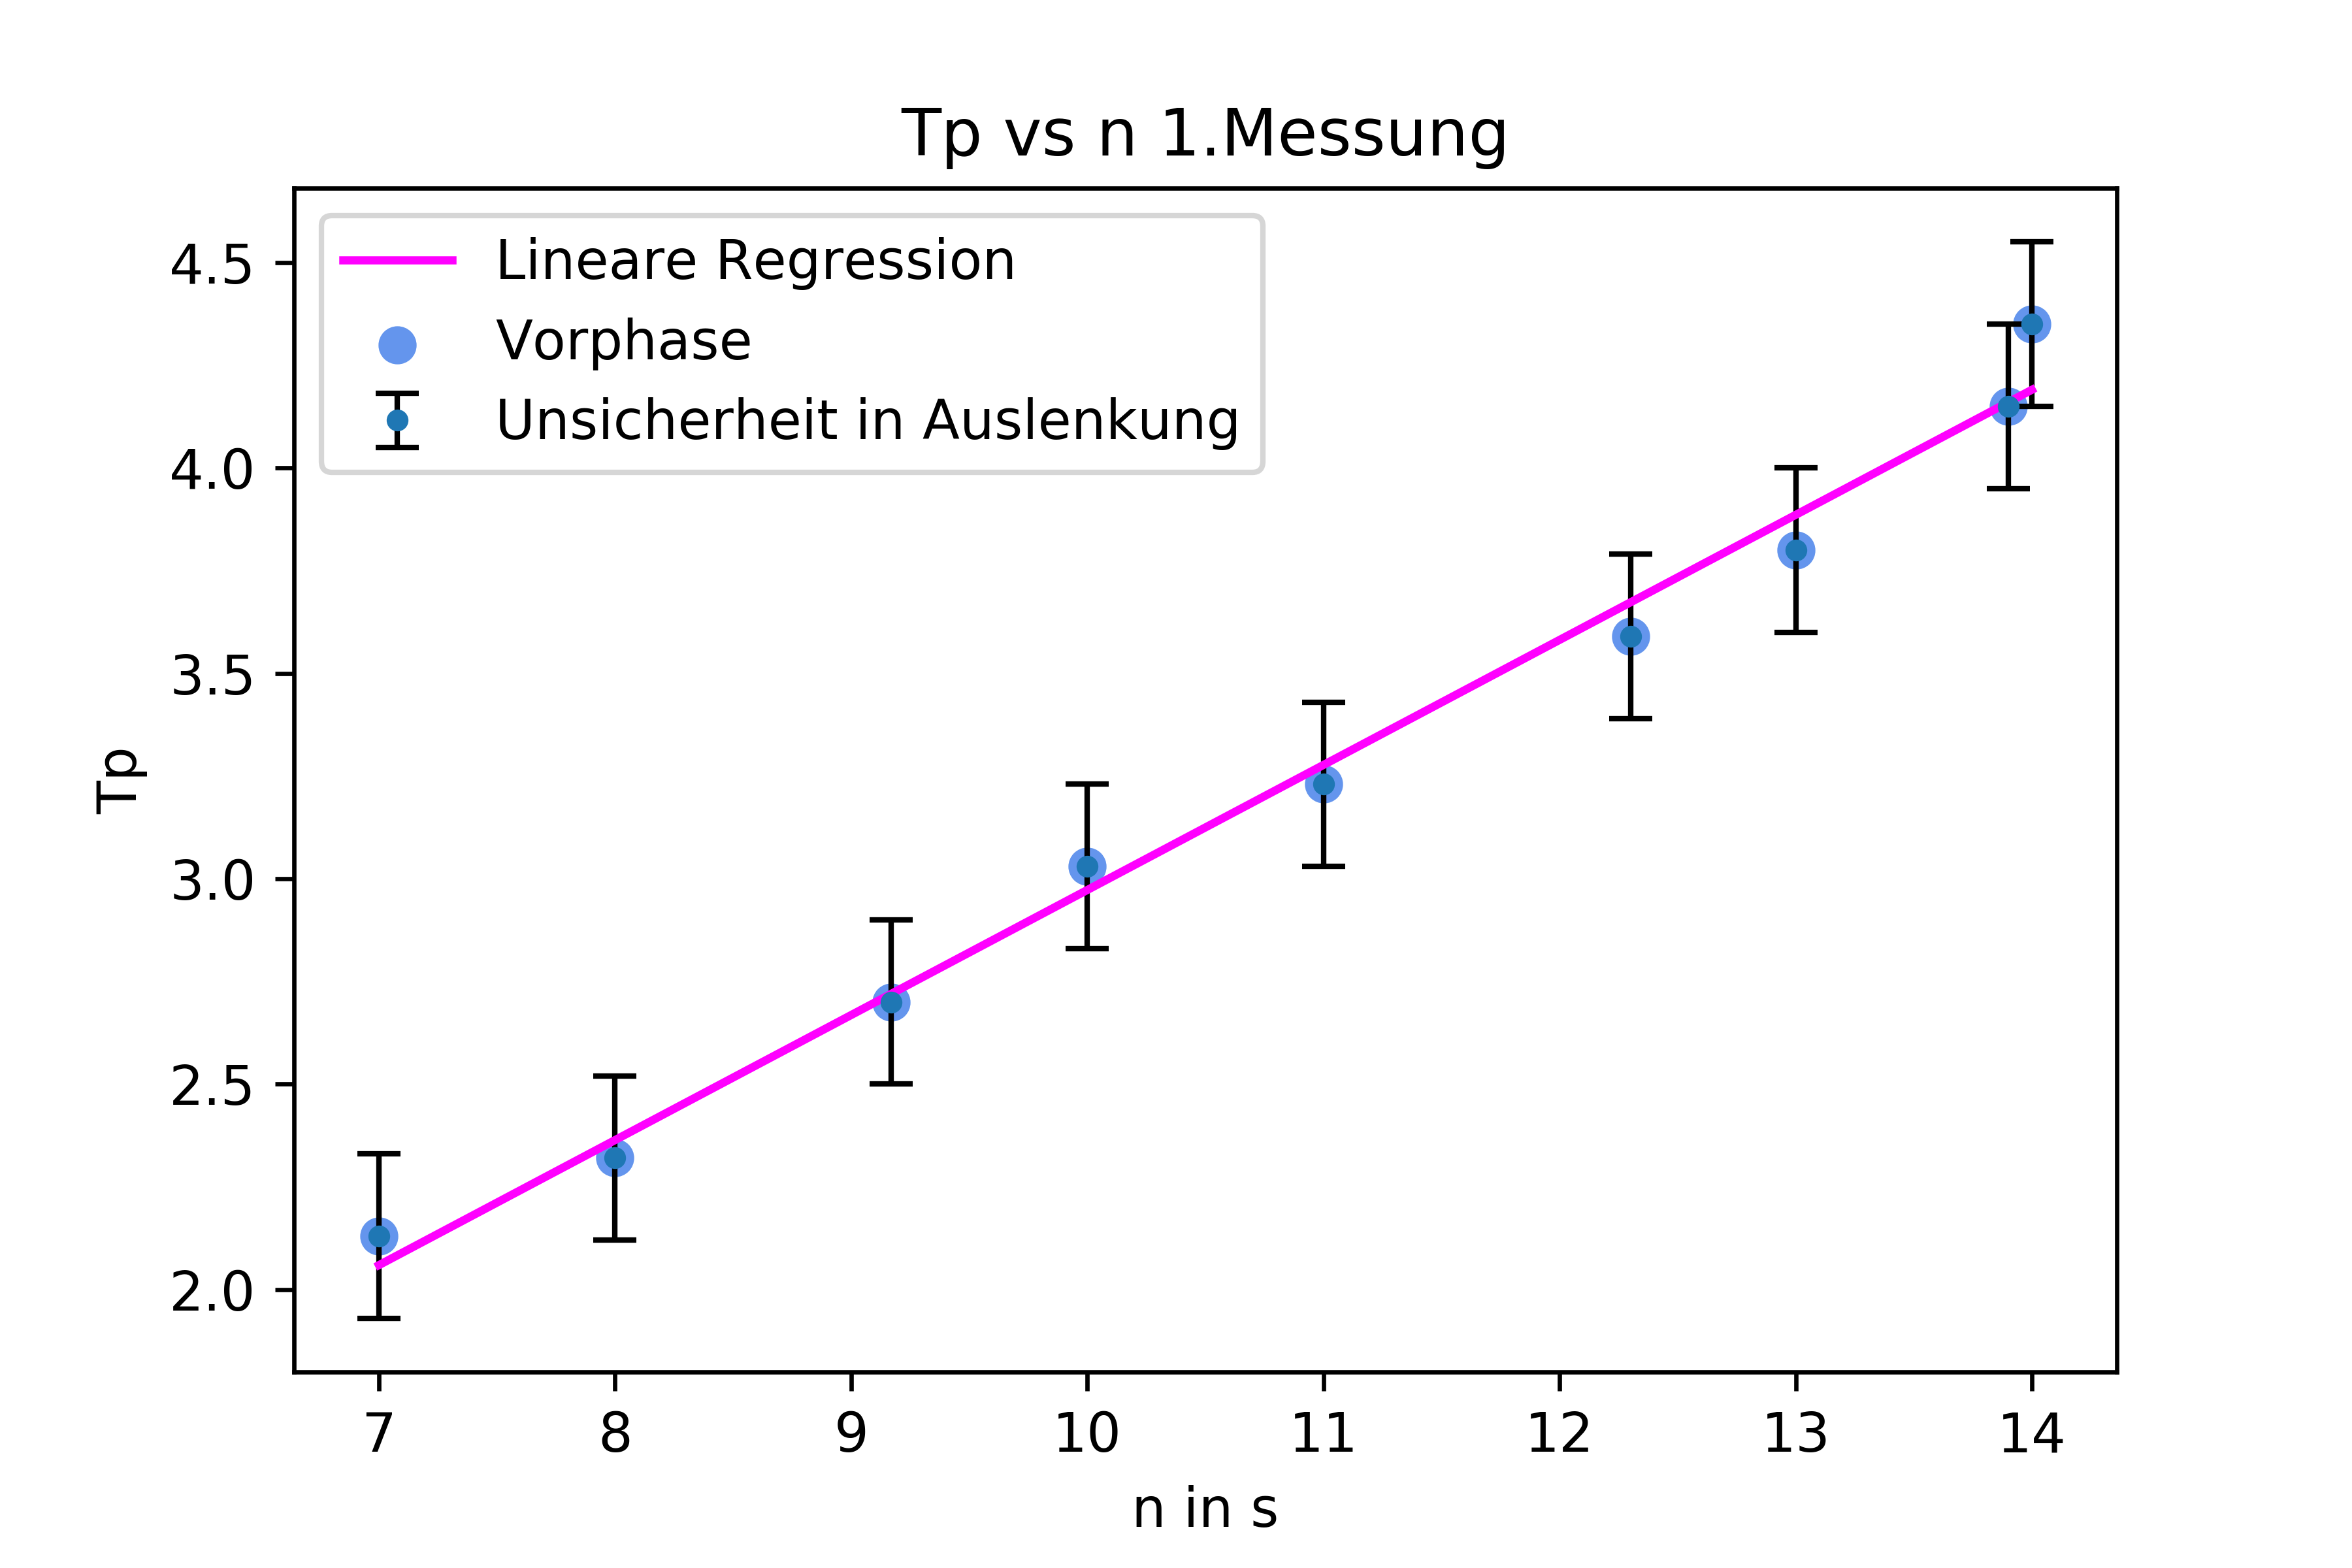
\includegraphics[width=300pt]{fotos/gpr1/M10_A2_S.png}
	\caption[Präzesion in Abhängigkeit der Kreisdrehzahl]{Präzesion in Abhängigkeit vom Drehmoment; $ a=0.304\pm 0.012 $ sei die Steigung, $ b= -0.2\pm 0.4$ der Achsenabschnitt, $ \chi^{2}/dof=0.75 $ Qualtität des Fits}							 
	\label{Abb: A2 Sara}							 
\end{figure}
	Der lineare Zusammenhang wurde somit bestätigt
\subsection{$ J_{x} $ Berechnung}
Aus der Steigung ergibt sich die Formel für den $ J_{x} $-Wert:
\begin{equation}\label{eq: Jx A2}
	J_{x}=\dfrac{a\cdot M}{4 \pi ^{2}}
\end{equation}
Damit ergeben sich folgende $ J_{x} $-Werte
\begin{table}[ht!]
	\centering
	\caption[Trägheitsmoment]{$ J_{x} $ aus der Gleichung (\ref{eq: Jx A2})}
	\begin{tabular}{|c|c|c|}
		\hline
		& Experimentatorin & Experimentator \\
		\hline
		$ J_{x} $ [kg m$ ^{2} $]& $ ( 2.477\pm0.027 ) $ & $ (2.42\pm0.11) $ \\
		\hline
	\end{tabular}
	\label{tab: Jx A2}
\end{table}


	
	\section{Nutationbewegung}
	\subsection{Datenauswertung}\label{sect: Datenauswertung A3}
	Für den Radius siehe Kapitel \ref{sect: Datenauswertung A1}.\\
	Damit wird die lineare Regression gemäß Material 2 der Form $ y=mx+b $.
	Daraus ergibt sich:
	\begin{equation}\label{eq: Tn A3}
		T_{n}=\dfrac{J_{s}}{J_{x}}\dfrac{1}{n}=\dfrac{a}{n}+b
	\end{equation}
	Mit a der Anstieg des Graphen und b die Periodendauer bei einer unendlich Kreiseldrehzahl durch die Nutationsbewegung entsteht.
	
	
	\begin{figure}[!ht]
		\centering								 
		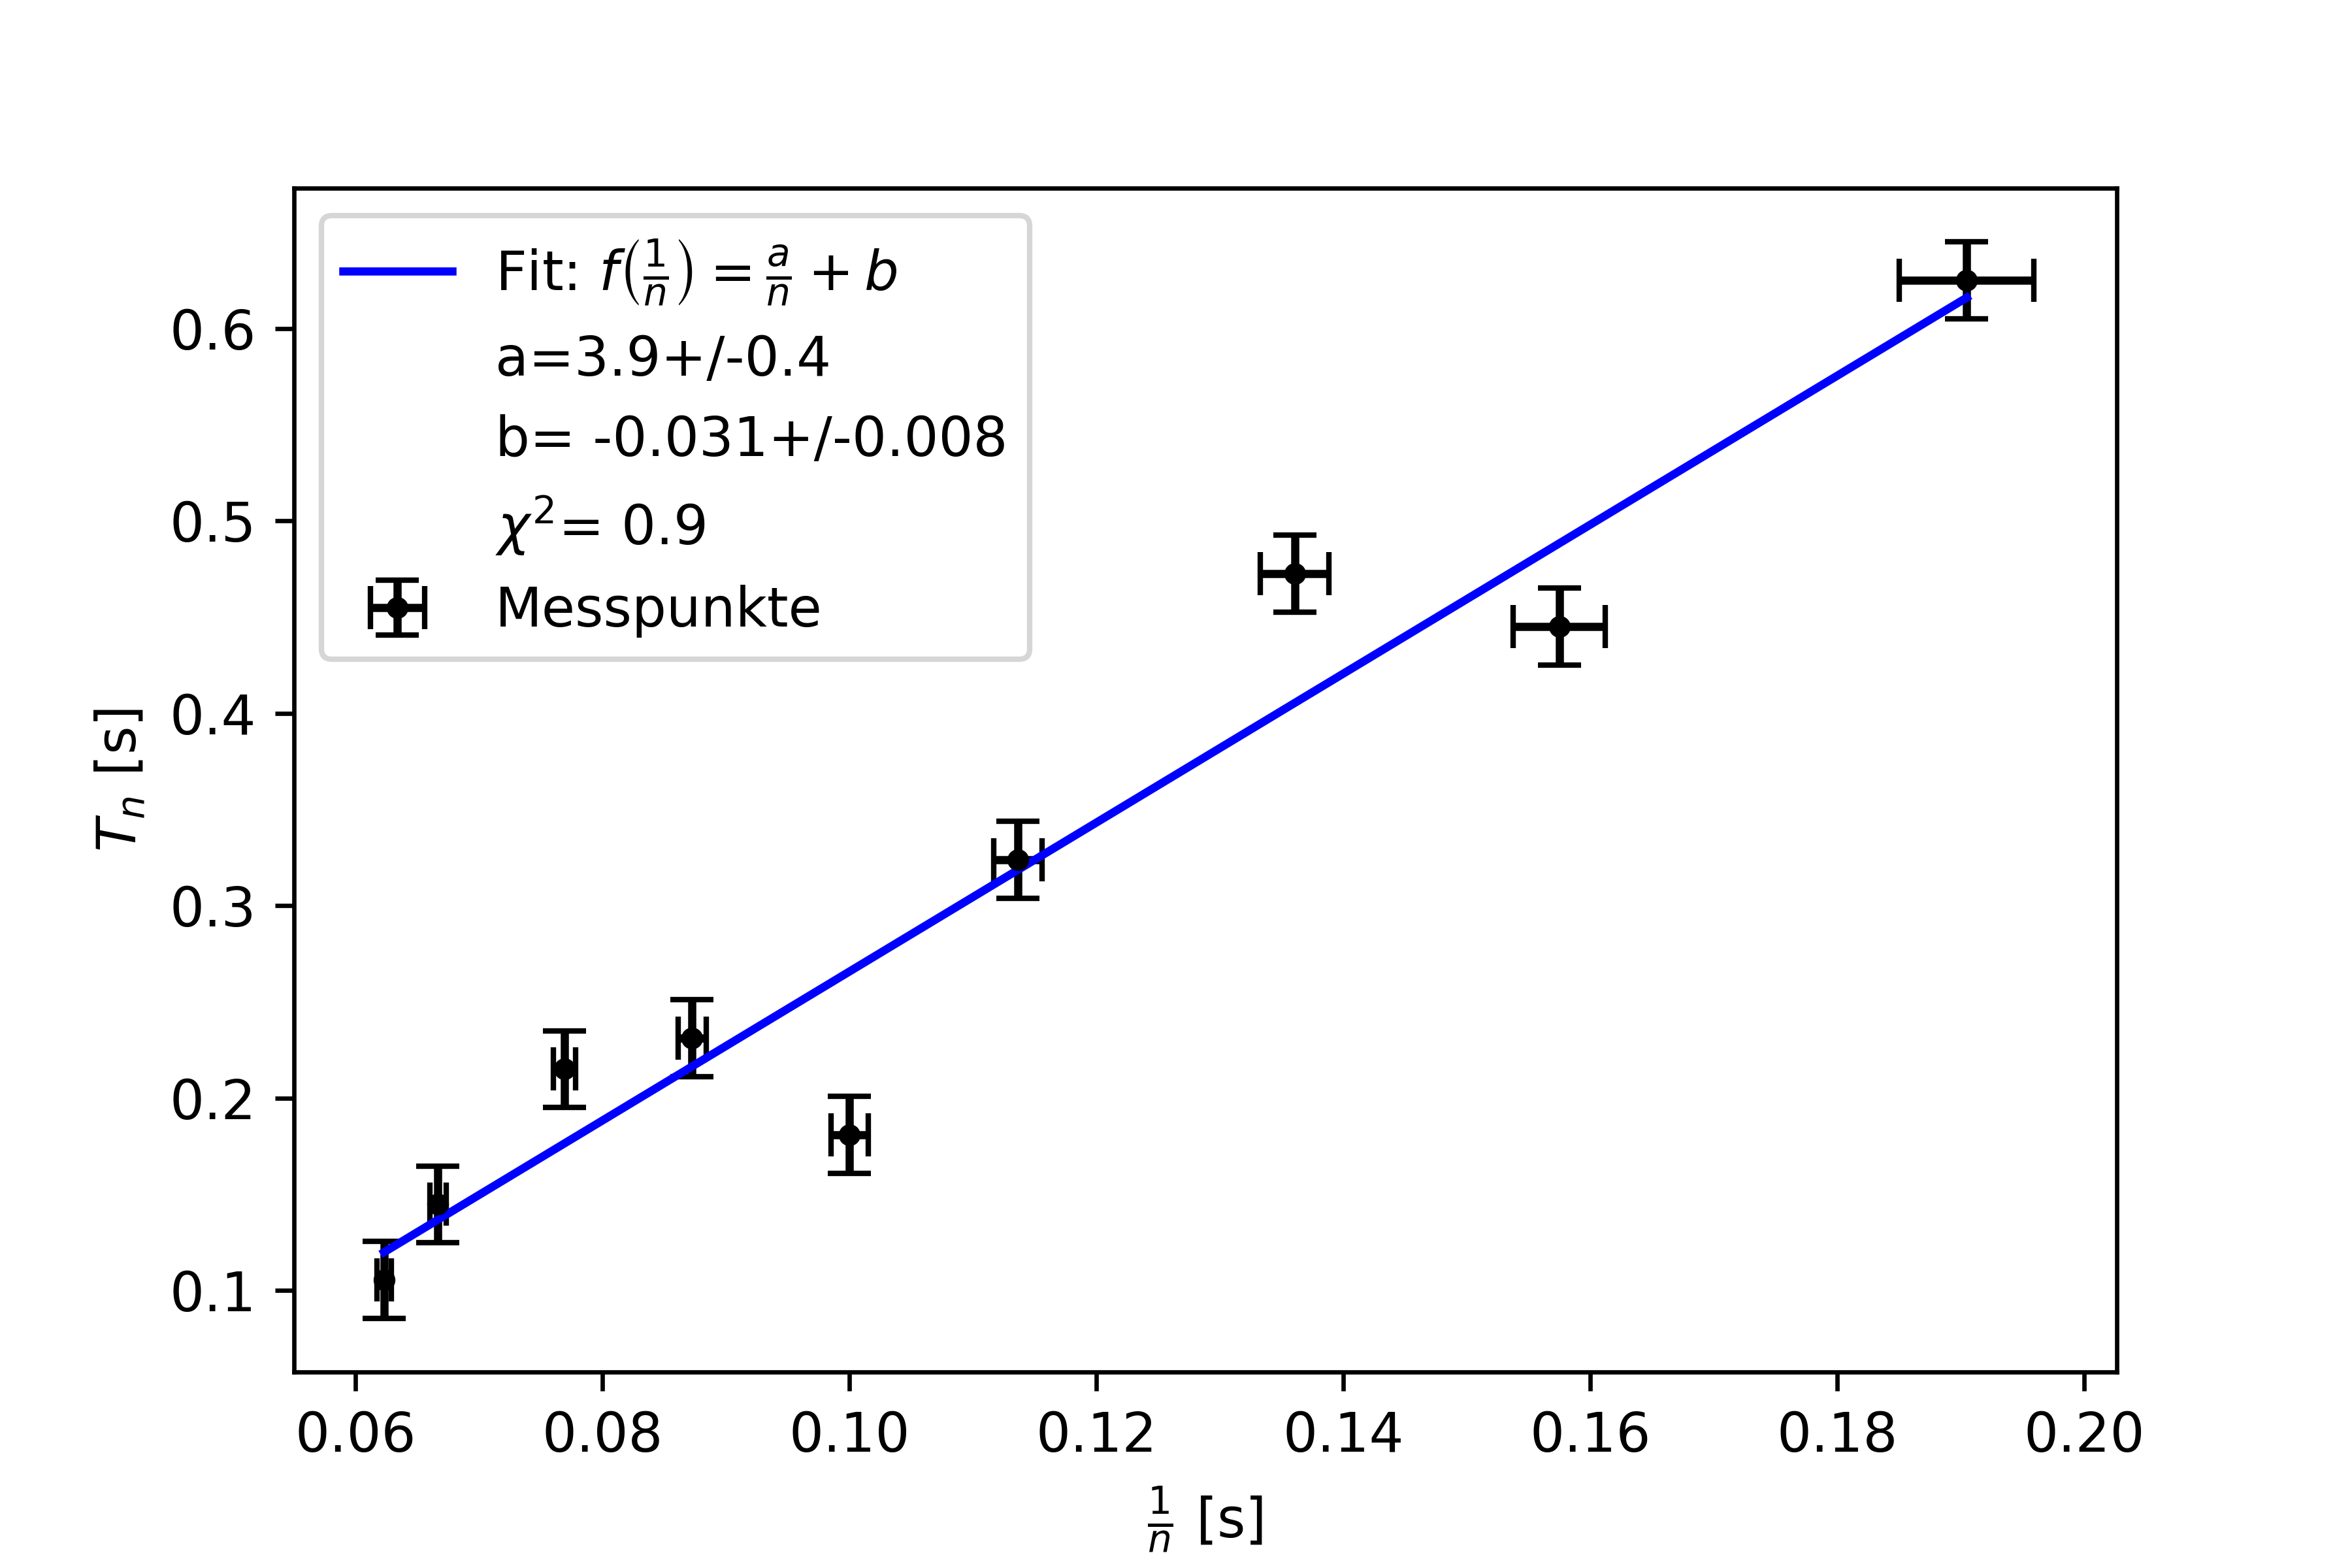
\includegraphics[width=300pt]{fotos/gpr1/B_A3.png}
		\caption[Nutation in Abhängigkeit der Kreisdrehzahl]{Nutation in Abhängigkeit vom Drehmoment, Ben F.; $ a $ sei die Steigung, $ b $ der Achsenabschnitt, reduziertes $ \chi^{2} $: Qualtität des Fits}							 
		\label{Abb: A3}							 
	\end{figure}
	
	
	\newpage
	\begin{figure}[!ht]
		\centering								 
		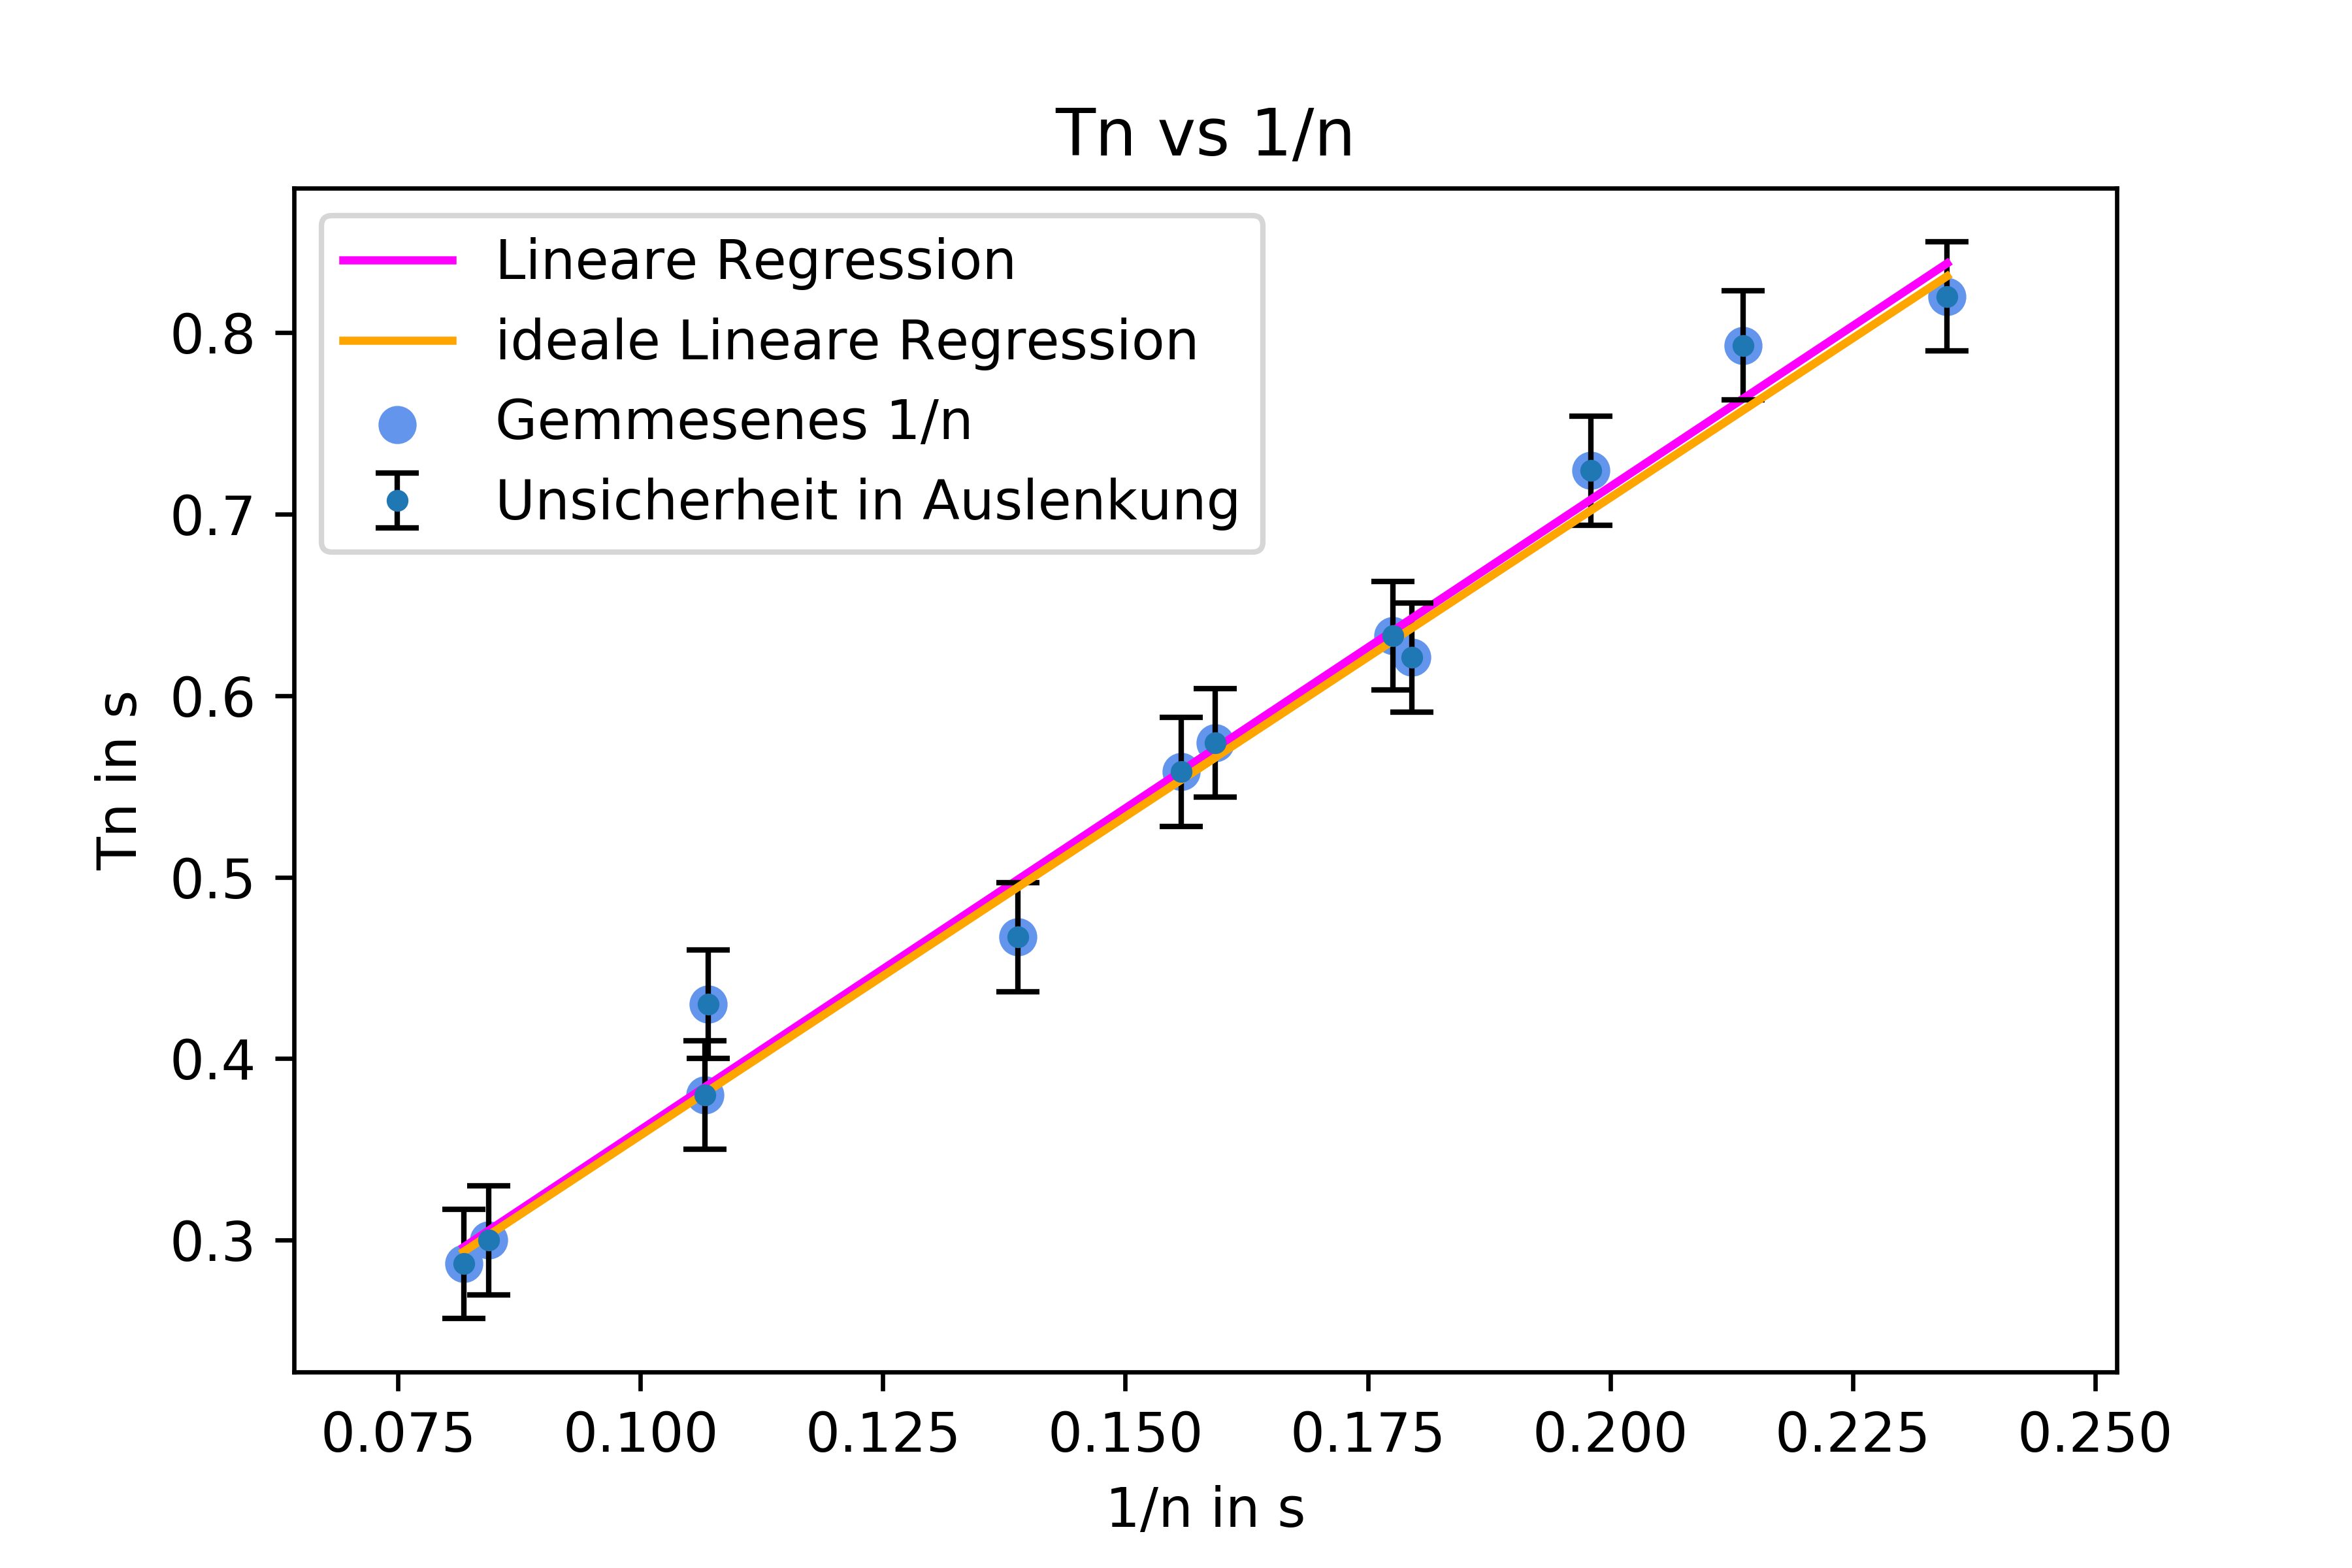
\includegraphics[width=300pt]{fotos/gpr1/M10_A3_S.png}
		\caption[Präzesion in Abhängigkeit der Kreisdrehzahl]{Präzesion in Abhängigkeit vom Drehmoment; $ a=3.45\pm 0.13 $ sei die Steigung, $ b=0.002\pm 0.006 $ der Achsenabschnitt, $ \chi^{2}/dof=0.56 $ Qualtität des Fits}							 
		\label{Abb: A3 Sara}							 
	\end{figure}
	
	Der lineare Zusammenhang wurde somit bestätigt.
	\subsection{$ J_{s} $ Berechnung}
	
	Aus der Steigung ergibt sich der $ J_{s} $-Wert wie folgt:
	\begin{equation}\label{eq: Js}
		J_{s}=J_{x}a
	\end{equation}

	Dabei nehmen wir als $ J_{x} $-Wert das gewichtete Mittel:
	
	\begin{table}[ht!]
		\centering
		\caption[Mittelung von $ J_{x} $]{gewichtetes Mittel von $ J_{x} $}
		\begin{tabular}{|c|c|c|}
			\hline
			& Experimentatorin & Experimentator \\
			\hline
			Mittelung von  $ J_{x} $ [kg m$ ^{2} $]& $(2.477 \pm0.029)\cdot 10^{-3} $ & $ (2.37\pm0.11)\cdot 10^{-3} $ \\
			\hline
		\end{tabular}
		\label{tab: Jx gemittelt}
	\end{table}
	
	Aus der Gleichung (\ref{eq: Js}) ergeben sich folgende Werte:
	
	\begin{table}[ht!]
		\centering
		\caption{Ergebnisse zu $ J_{s} $}
		\begin{tabular}{|c|c|c|}
			\hline
			& Experimentatorin & Experimentator \\
			\hline
			Ergebnisse $ J_{s} $ [kg m$ ^{2} $]& $(8.7 \pm0.3 )\cdot 10^{-3}$ & $  (10.3 \pm1.2)\cdot 10^{-3} $ \\
			\hline
		\end{tabular}
		\label{tab: Ergebnisse Js}
	\end{table}
	
	
	
	\newpage
	\section{Berechnung von $ J_{x} $}
	Das Trägheitsmoment des Kreisels ergibt sich durch Unterteilung des Kreisels in Hohlzylinder.
	Das Trägheitsmoment des Gyroskop ergibt sich unter der Betrachtung des Gyroskop als Zusammensetzung verschiedener Hohlzylinder. Die Abmessungen sind aus den Skizzen (\ref{Abb: Längenskizze Platz 2}) und (\ref{Abb: Längenskizze Platz 4}) zu entnehmen. Zu beachten ist, dass das Tarriergewicht und die Schraube ebenfalls einen Beitrag leisten. Als Fehler der Abmessungen nehmen wir den Wert $ 0.05 $mm. Die einzelnen Hohlzylinder werden mit der folgenden Formel berechnet:
	\begin{equation}\label{eq: Berechnung von Jx}
		J=\dfrac{1}{2}\rho \pi h (r^{4}_{2}-r^{4}_{1})
	\end{equation}
	Bei der Dichte $ \rho $ muss beachtet werden, dass der Eisenträger eine andere Dichte aufweißt als die anderen Teile des Gyroskop aus Messing. Die Dichten sind im Versuchsskript\smartcite{Muller.d} nach zu lesen.\\
	Nach der Addition der Trägheitsmomente der einzelnen Trägheitsmomente der Hohlzylinder bekommen wir folgende Werte für $ J_{x} $:
	\begin{table}[ht!]
		\centering
		\caption[Ergebnisse]{Ergebnisse der Berechnung von $ J_{x} $}
		\begin{tabular}{|c|c|c|}
			\hline
			& Experimentatorin & Experimentator \\
			\hline
			$ J_{x} $ [kg m$ ^{2} $]&$  3.097\pm 0.009 $ & $ 2.671\pm 0.009 $ \\
			\hline
		\end{tabular}
		\label{tab: Berechnung von Jx}
	\end{table}
	
	
	
	
	
	
	
	
	
	
	
	
	
	\section{Vergleich}
	Im Experiment wurden folgende Werte für die Hauptträgheitsachsen gemessen oder als theoriewert angegeben/errechnet.
	
	\begin{table}[ht!]
		\centering
		\caption[Vergleich]{Vergleich der Theoretischen und experimentellen $ J_{s} $}
		\begin{tabular}{|c|c|c|}
			\hline
			& Experimentatorin & Experimentator \\
			\hline
			Theoriewert $ J_{s} $ [kg m$ ^{2} $] & $ (8.7 \pm 0.5) $ & $ 9.7\pm0.5 $ \\
			\hline
			Experimentaler Wert $ J_{s} $ [kg m$ ^{2} $] & $(8.7 \pm0.3 )\cdot 10^{-3}$ & $(10.3 \pm1.2)\cdot 10^{-3} $  \\
			\hline
		\end{tabular}
		\label{tab: Vergleich}
	\end{table}
	
	
	
	Das gewichtete Mittel und der theoretisch berechnete $ J_{x} $ Wert decken sich in ihren Unsicherheitsbereichen. Was auffällt, dass bei der ersten Messreihe der Wert geringer ist und sich nicht mit dem Unsicherheitsbereich des Theoriewertes überschnitten.
	Der $ J_{s} $ Wert hingegen scheinen genau übereinzustimmen, der gemessene Wert scheint sogar genauer zu sein.
	
	
	\newpage
	\section{Chi Quadrat}
	Zur Einschätzung der Genauigkeit der Messung kann man Chi Quadrat verwenden. Die Formeln dazu
	findet man im Skript \textit{Physikalische Grundlagen}\smartcite{MullerPG.2007b}.
	
	\begin{table}[ht!]
		\centering
		\caption{reduzierte $ \chi^{2} $}
		\begin{tabular}{|c|c|c|c|}
			\hline
		Messung	& & Experimentatorin  & Experimentator \\
			\hline
		Präzision (Drehmoment)& 	$ \chi^{2}/dof $& 0.69 &0.39  \\
			\hline
			Präzision (Kreisdrehzahl)& 	$ \chi^{2}/dof $& 0.35 & 0.49 \\
			\hline
			Nutation& 	$ \chi^{2}/dof $& 0.56  & 0.9 \\
			\hline
		\end{tabular}
		\label{tab: chi quadrat}
	\end{table}

	Beim $ \chi^{2} $ wird für eine reelle Messung innerhalb des Praktikums ein Wert von 1 erwartet.
	Bei den Experimenten liegen die $ \chi^{2} $'te nahe dem Erwartungswert, da diese für 10 Datenpunkte im
	Bereich einer guten Messung sind. Aufgrunddessen wurden die Fehler als niedrig eingeschätzt, trotz ihrer Größe.
	Bei dem ersten Versuch ergab sich ein niedriger Wert auf Grund genauer Messungen, da die
	Messpunkte nahe des Fits sind.\\\\
	Beim Experimentator waren die Werte der ersten beiden Messungen ähnlich wie bei der
	Experimentatorin niedrig aber verhältnismäßig gegenüber den Anzahl der Messdaten.
	Bei der dritten Messung ist das $ \chi^{2} $ etwas unter 1, aber im guten Bereich, was bedeutet, dass die Fehler gut
	abgeschätzt sind. Trotz Streuung sind die Messdaten im statistischen erwarteten Bereich und ziehen die
	Ergebnisse nicht runter. 
	
	\section{Fehlereinschätzung}
	\subsection{Fehlerfreie Werte}
	Es wurde angenommen, dass werte wie die Dichte oder die Gravitationskonstante fehlerfrei sind, die sind jedoch ebenso fehlerbehaftet. Jedoch sind die Fehler so klein, dass diese bei der Rundung vernachlässigt worden wären, somit vernachlässigt werden können
	\subsection{Kleinwinkelnäherung}
	Einer der größten Fehlerquellen war mit unter die Kleinwinkelnährung. Dabei haben wir angenommen, dass es keinen, oder vernachlässigbar kleinen Winkel, zur ursprünglichen $ x $-Achse gibt.
	Bei kleinen Massen war dies leicht zu erreichen, wenn auch mit Augenmaß, somit dort vernachlässigbar. Bei größeren Massen hingegen war es sehr schwer zu erreichen und nur durch anstupsen zu erreichen, was jedoch die Werte ebenso verfälschen kann.
	So konnte auch nur ca. 1 Periode gemessen werden, da sich der Kreisel immer mehr zu neigen begann mit der Zeit und bei höheren Masse.
	Dies würde den $ J_{x} $ Wert vergrößern.
	\subsection{Nicht konstante Kreisdrehzahl}
	Besonders am Platz 2 gab es anfänglich starke Schwankungen der Kreiseldrehzahl, was es sehr schwierig machte diese zu messen. So konnte nur die Zeit für eine Periode gemessen werden, da sonst die Schwankungen zu groß waren. Nach mehreren malen wurden die Werte genommen wo es nur eine Schwankung von höchstens 0.5 Hz gab, um zu große Abweichungen zu vermeiden, da diese sonst stark ins Gewicht fielen. So wurde auch die größte Abweichung von dem gemessenen n Wert genommen und der n Wert, als der aufgeführt, in dessen Bereich während des Experimentes die Kreisdrehzahl am meisten war
	\subsection{Zeitmessung}
	Bei der Messung der Periodendauer der Präzisionsbewegung wurde eine digitale Stopuhr genutzt. Dort muss man neben den Gerätefehler noch zweimal die Reaktionszeit von ca. 0.25s als Unsicherheit genommen. Die sind bei den kleinen Zeiten die man gemessen hatte so groß, dass kaum der Geräte beachtet werden musste.\\
	\\
	Bei der Nutationsbewegung wurde ein Video aufgenommen und über ein Videobearbeitungsprogramm die Periodendauer gemessen. Dies sorgt dafür, dass man die Reaktionszeit nicht braucht und die Werte genauer werden. Generell scheint dieses Verfahren sehr vorteilhaft, wenn man sehr kleine Periodendauern zu messen hat.
	So wurde die Unsicherheit hier auf 0.02s ca. geschätzt da in diesen Bereich das Video ausgewertet wurde.\\
	Der Experimentator hat bei der Nutationsbewegung sowohl die Zeit über die Stoppuhr als auch die Nutationsbewegung mit dem Smartphone\footnote{mit Android-Betriebssystem} auf Video aufgenommen. Danach wurde das Video mit Hilfe eines Videobearbeitungsprogramm um das fünfache verlangsamt und die Zeit abgelesen. Die Reaktionszeit lässt sich dann wie folgt berechnen: $ u_{Reaktionszeit}=1.2/2 \text{ [s] }=0.6 \text{ [s] }$
	\subsection{Reibung}
	Wie im jeden realen Versuch gibt es Reibung.
	Da jedoch der Motor den Kreisel auf eine bestimmte Drehzahl brachte und man nur kleine Periodendauern gemessen hatte, hatte die Reibung kaum einen Effekt und konnte vernachlässigt werden.
	
	
	
	\section{Schlussfolgerungen}
	Generell kann man das Experiment als gelungen betrachten werden, da trotz der hohen Anfälligkeit von Unsicherheiten durch dem ungenauem einstellen der Kreiseldrehzahl, wurden die Theoriewerte nahezu erreicht. Nur bei der ersten Messung war der Wert niedriger, was von vorzeitigen Stoppen zusammen mit den schwankenden n Werten verursacht worden sein konnte.
	Außerdem wurden die linearen zusammenhänge bestätigt.\\\\
	Durch bessere Motoren und erzeugen eines genaueren Kreiseldrehzahlen würden die Messungen ebenso genauer werden. Außerdem würde eine Masse bis zu 400 g vorteilhaft sein, da bei 500g und 450 g es einen zu großen Winkel für die Kleinwinkelnährung gibt und man erst diesen anstupsen musste, was zu einer Verfälschung der Werte führen könnte.\\\\
	Ebenso hat sich die Methode mit der Videobearbeitung als sehr hilfreich erwiesen und scheint eine sehr effektive Methode zur Messung von kleinen Periodenzeiten zu sein. Dies wäre eine besser alternative als Lichtschranken, da sich durch das Gewicht der Masse die Achse zu neigen beginnt bei der Präzision und bei der Nutation der Radius der Drehung immer kleiner wird, wodurch sich eine Lichtschranke nicht zu eigenen scheint, um die Reaktionszeit auszugleichen.
	
	
	
	
	\newpage
    \appendix
	\section{Anhang}
	
	\subsection{zusätzliche Skizzen}\label{sect: Zusätliche Skizzen}
	
	\begin{figure}[!ht]
		\centering								 
		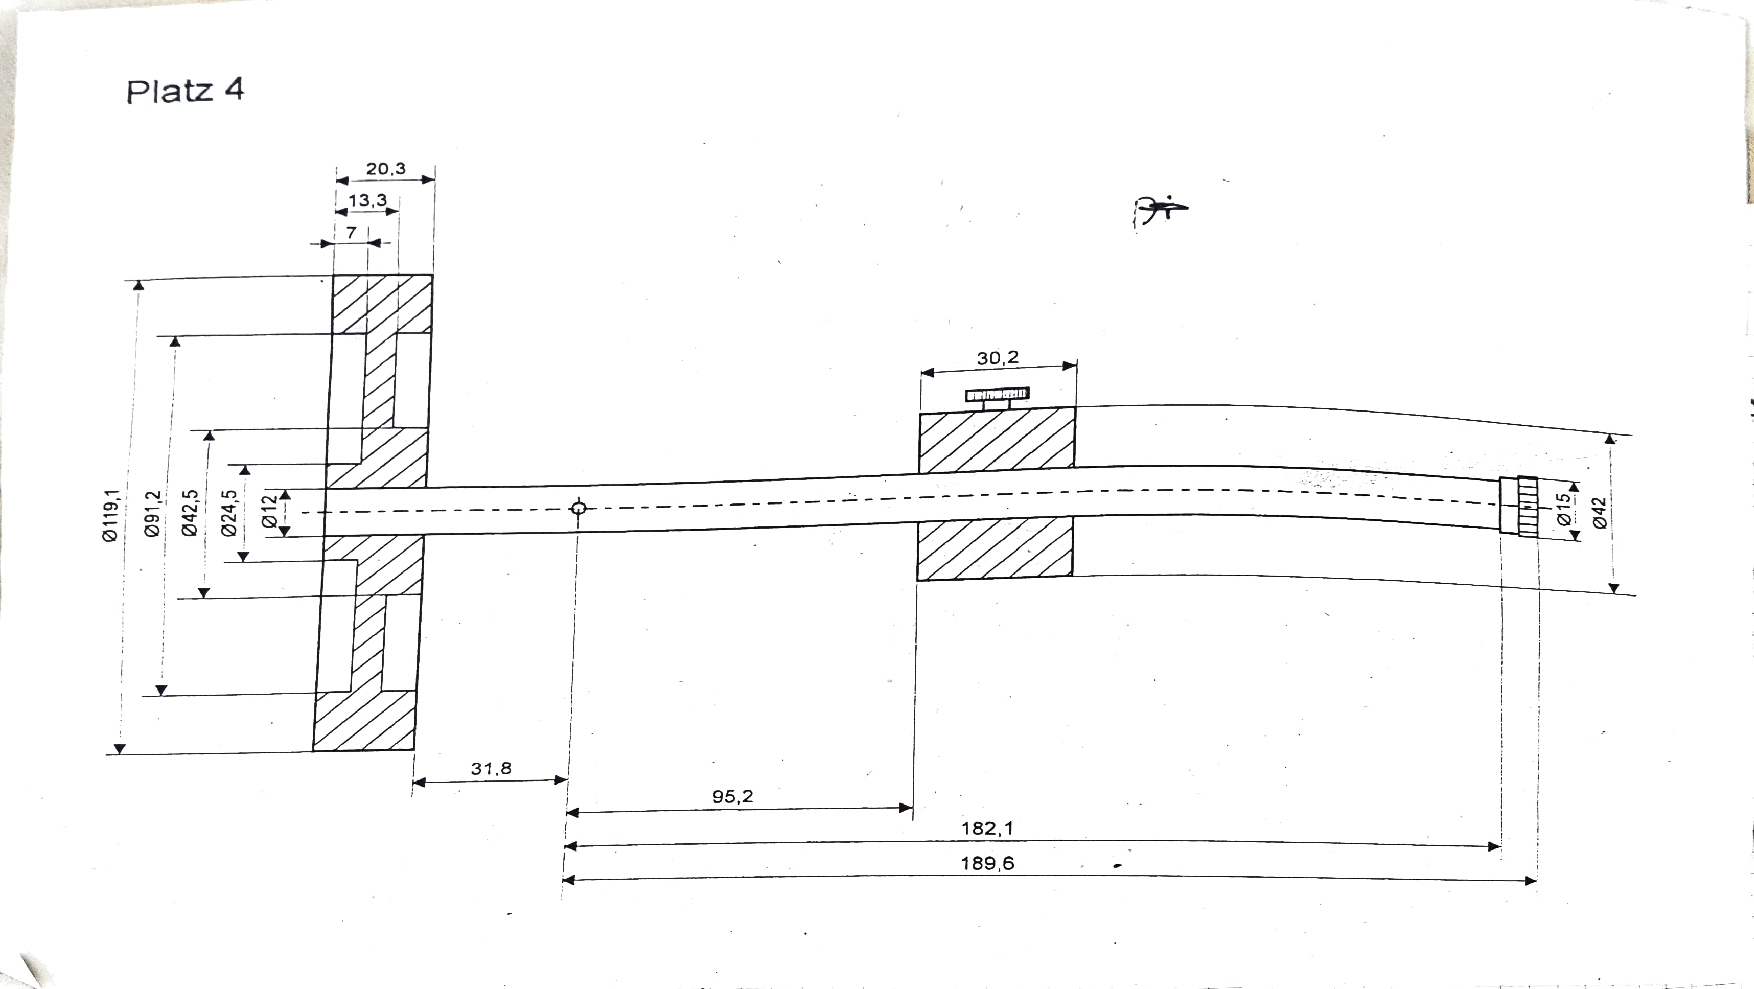
\includegraphics[width=300pt]{fotos/gpr1/M10.Skizze.pdf}			 
		\caption[Längenskizze Gyroskop, P4]{Längenskizze des Gyroskop, wichtig für das Drehmoment des Gyroskop bzgl. $ r $, Messplatz 4}							 
		\label{Abb: Längenskizze Platz 4}							 
	\end{figure}
	
		\begin{figure}[!ht]
		\centering								 
		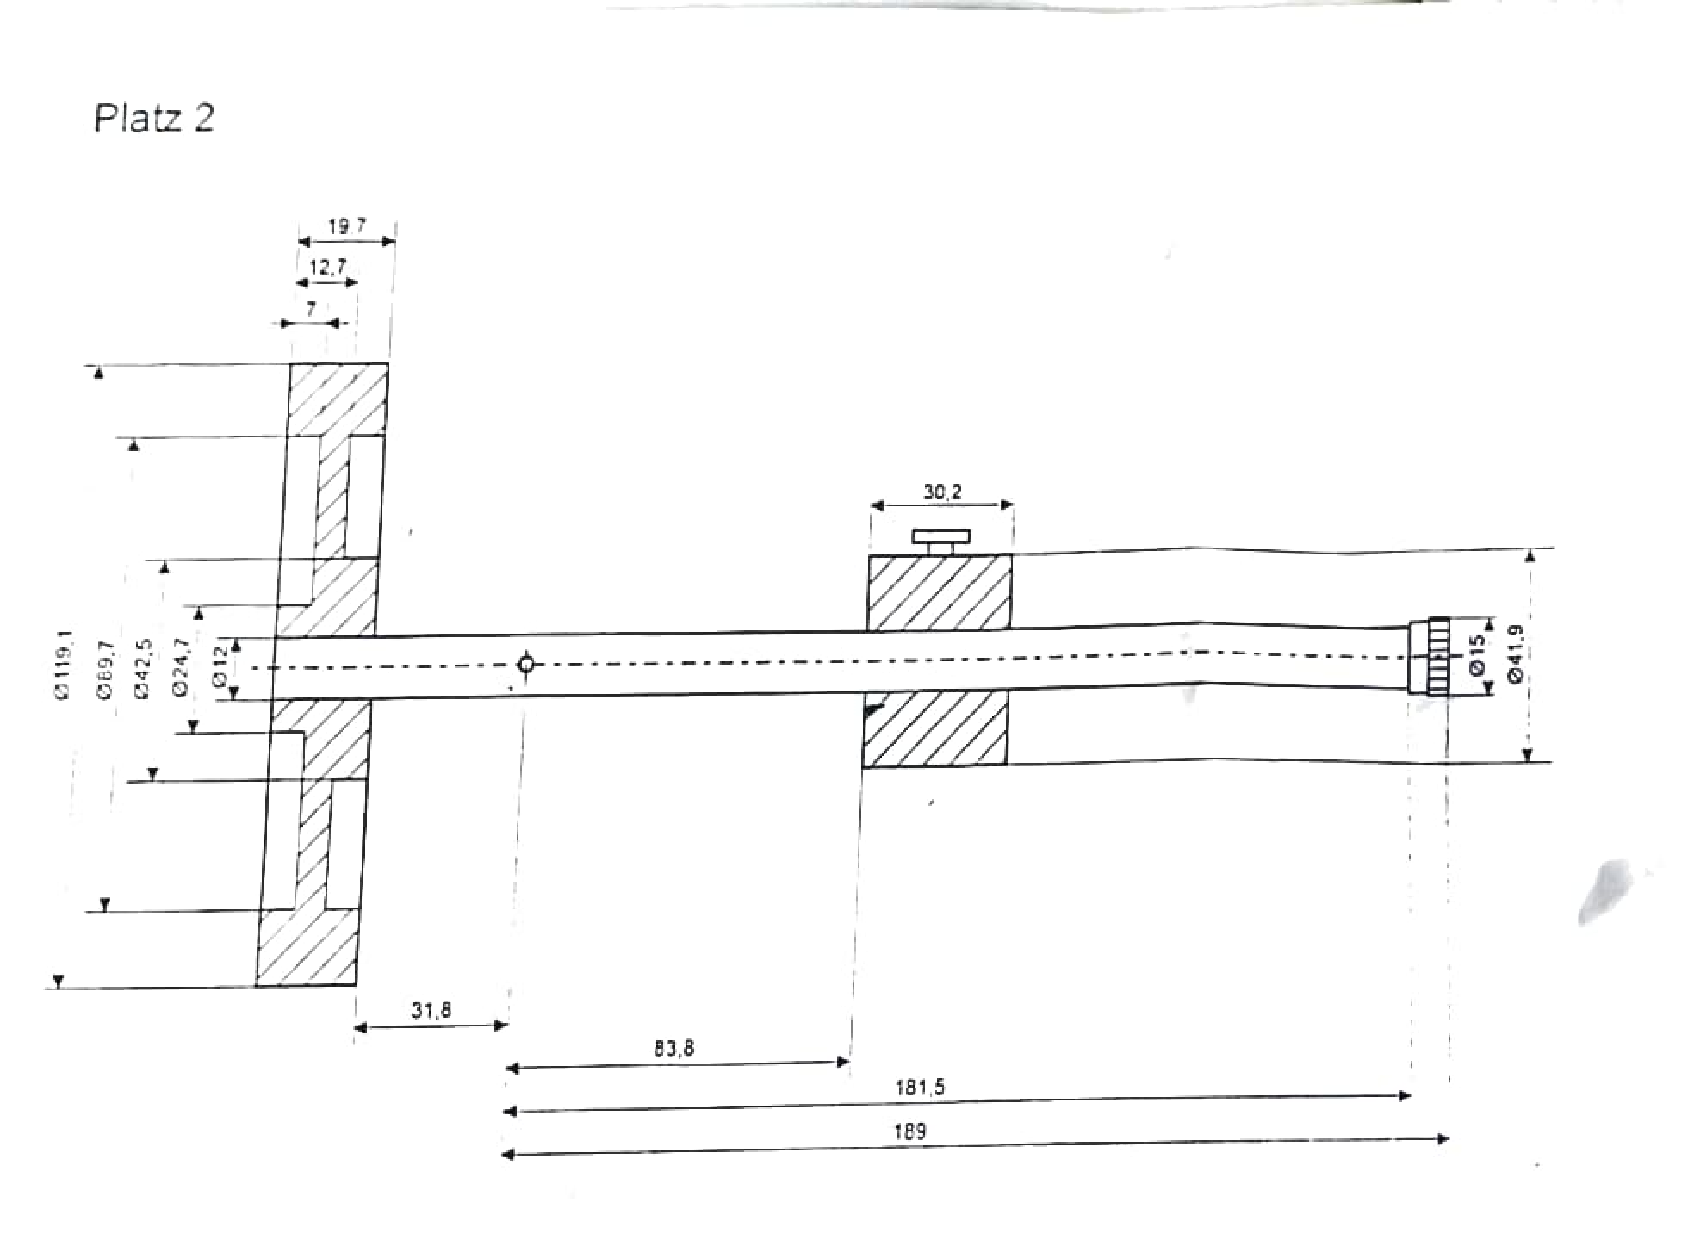
\includegraphics[width=300pt]{fotos/gpr1/M10_S2.pdf}			 
		\caption[Längenskizze Gyroskop, P2]{Längenskizze des Gyroskop, wichtig für das Drehmoment des Gyroskop bzgl. $ r $, Messplatz 2}							 
		\label{Abb: Längenskizze Platz 2}							 
	\end{figure}
	
	
	
	\newpage
	\subsection{Versuchsaufzeichnungen}
	
	\begin{table}[ht!]
		\centering
		\caption[Versuchsaufzeichungen]{Versuchsaufzeichungen\\ der Nutationsmessreihe}
	\begin{tabular}{|c|c|}
		\hline
		n &     T \\
		\hline
		0.234742 & 0.820 \\
		0.213675 & 0.793 \\
		0.198020 & 0.724 \\
		0.179533 & 0.621 \\
		0.177620 & 0.633 \\
		0.155763 & 0.558 \\
		0.159236 & 0.574 \\
		0.138889 & 0.467 \\
		0.106952 & 0.430 \\
		0.106610 & 0.380 \\
		0.084317 & 0.300 \\
		0.081766 & 0.287 \\
		\hline
	\end{tabular}
	\label{tab: Nutationswerte}
	\end{table}

	\newpage
	\printbibliography[title={Quellenverzeichnis}]
	
	
\end{document}